
\seccion{Entrop\'ia como medida de incerteza}
\label{s:SZ:Entropia}

% ================================= Axiomas

\subseccion{Entrop\'ia de Shannon, propiedades}
\label{sec:SZ:DefinicionShannon}

Un de los primeros trabajos  tratando de formalizar la noci\'on de informaci\'on
de una cadena  de simbolos es debido a Raph  Hartley~\cite{Har28}.  En su papel,
Hartley defin\'o la informaci\'on de una secuencia como siendo proporcional a su
longitud. Mas precisamente,  para simbolos de un alfabeto  de cardinal $\alpha$,
exiten  $\alpha^n$   cadenas  diferentes  de   longitud  $n$;  Se   defin\'o  la
informaci\'on de tales cadenas como  siendo $K n$ ($K$ dependiente de $\alpha$).
Para  ser  consistente,  dos   conjuntos  de  mismo  tamanio  $\alpha_1^{n_1}  =
\alpha_2^{n_2}$   deben  llegar  a   la  misma   informaci\'on,  as\'i   que  la
informaci\'on de Hartley es definida como $H = \log\left( \alpha^n \right)$ donde
la base del logaritmo es arbitraria.  Dicho de otra manera, tomando un logaritmo
de  base 2,  esta  informaci\'on  es nada  mas  que los  numeros  de bits  (0-1)
necesarios para  codificar todas las cadenas  de longitud $n$ de  simbolos de un
alfabeto de cardinal $\alpha$.

\SZ{Hartley, equiv de Gibbs de la termostat}.

Una debilidad del  enfoque de Hartley es que considera  implicitamente que en un
mensage, cada cadena de longitud dada  puede aparecer con la misma frecuencia, o
probabilidad $1/\alpha^n$,  siendo la informaci\'on menos el  logaritmo de estas
probabilidades.  A contrario, parece  mas l\'ogico considerar que secuencias muy
frecuentes no  llevan mucha informaci\'on  (se sabe que aparecen),  mientras que
las  que aparencen  raramente llevan  mas informaci\'on  (hay mas  sorpresa, mas
incerteza  en observarlas).  Volviendo  a los  simbolos elementales  $x$, vistos
como aleatorios (o valores o estados que puede tomar una variable aleatoria), la
(falta  de)  informaci\'on o  incerteza  va a  ser  intimamente  vinculada a  la
probabilidad de aparici\'on de estos simbolos $x$. Siguiendo la idea de Hartley,
la informaci\'on elemental  asociado al estado $x$ va a ser  $- \log p(x)$ donde
$p(x)$  es la  probabilidad de  apararici\'on de  $x$.  Se  define  la incerteza
asociada a  la variable aleatoria como  el promedio estadistico  sobre todos los
estados  posibles $x$~\cite{Sha48, ShaWea64}~\footnote{En  la misma  \'epoca que
  Shannon,  independientemente,   la  noci\'on  de   informaci\'on  o  medidades
  equivalentes apareciendo por ejemplo en calculo de capacidad de canal aparecen
  en  varios  trabajo  como  el de  Calvier~\cite{Cla48},  Laplume~\cite{Lap48},
  Wiener~\cite[Cap.~III]{Wie48}  entre  varios  otros  (ver~\cite{Ver98,  Lun02,
    RioMag14, FlaRio16, RioFla17, Che17}).}.
%
% \cite{Sha48, ShaWea64}
\begin{definicion}[Entropia de Shannon]\label{def:SZ:Shannon}
  Sea $X$ una variable aleatoria definida  sobre una alpfabeto discreto $\X = \{
  x_1 , \ldots , x_\alpha \}$ de cardinal $\alpha = |\X| < + \infty$ finito. Sea
  $p_X$ la  distribuci\'on de probabilidad  de $X$, \ie  $ \forall \, x  \in \X,
  \quad p_X(x)  = \Pr[X  = x]$.  La entropia de  Shannon de  la variable  $X$ es
  definida por
  %
  \[
    H(p_X) = H(X) = - \sum_{x \in \X} p_X(x) \, \log p_X(x)
  \]
  %
  con la convenci\'on $0 \log 0 = 0$.
\end{definicion}

La base del logaritmo es arbitrario; si  es $\log_2$ el logaritmo de base 2, $H$
es en bits y si se usa el logaritmo natural $\ln$, $H$ es en nats.  {\it En este
  cap\'itulo, se usara  $H$ con el logaritmo correspondiente  sin especificar la
  base.  Si  es necesario  que tenga  una base $a  (\ne 1)$  dada, se  notara la
  entropia  corespondiente  $H_a$  y   se  especifiera  la  base  del  logaritmo
  $\log_a$}.  Fijense de que $\log_a x = \frac{\log x}{\log a}$, dando
%
\[
H_a(X)  =  H_b(X)  \log_a b
\]
%
En  lo  que  sigue, a\'un  que,  rigorosamente,  $H$  sea  una funci\'on  de  la
distribuci\'on  de  probabilidad  $p_X$  y  no  de la  variable  $X$,  se  usara
indistamente la notaci\'on $H(p_X)$ tal  como $H(X)$ seg\'un lo mas conveniente.
Ademas, $p_X$ podr\'a denotar  indistamente la distribuci\'on de probabilidad, o
el  vector  de probabilidad  $p_X  \equiv  \begin{bmatrix}  p_X(x_1) &  \cdots  &
  p_X(x_\alpha) \end{bmatrix}^t$.

$H$ tiene propiedades notables, que coresponden a las que se puede exigir de una
medida de incerteza~\cite{Sha48, ShaWea64, CovTho06, Rio07, DemCov91, Joh04}:
%
\begin{propiedades}
\item\label{prop:SZ:continuidad} {\it Continuidad:}  Vista como una funci\'on de
  \ $\alpha$ \ variables  \ $p_i = p_X(x_i)$, \ $H$ \  es continua con respeto a
  los $p_i$.
%
\setcounter{PropPermutacion}{\value{enumi}}
\item\label{prop:SZ:permutacion}   {\it  Invariance  bajo   una  permutaci\'on:}
  Obviosamente,  la  entropia  es  invariante  bajo  una  permutaci\'on  de  las
  probabilidades, \ie,
  %
  \[
  \mbox{para cualquier  permutaci\'on } \sigma:  \X \to \X, \quad  H(p_{\sigma(X)}) =
  H(p_X) \quad \mbox{con} \quad p_{\sigma(X)}(x) = p_X(\sigma(x))
  \]
  %
  lo que se  escribe tambi\'en $H(\sigma(X)) = H(X)$.   En particular, denotando
  $p_X^\downarrow$ la  distribuci\'on de probabilidades obtenida a  partir de $p_X$,
  clasificando las  probabilidades en orden  decreciente, $p_X^\downarrow(x_1) \ge
  p_X^\downarrow(x_2) \ge \cdots  \ge p_X^\downarrow(x_\alpha)$,
  %
  \[
  H(p_X^\downarrow) = H(p_X)
  \]
%
\setcounter{PropBiyeccion}{\value{enumi}}
\item\label{prop:SZ:biyeccion}   {\it  Invariance   bajo   una  transformaci\'on
    biyectiva:}  La  entropia  es  invariante  bajo  cualquier  transformaci\'on
  biyectiva, \ie
  %
  \[
  \mbox{para cualquier  funci\'on biyectiva } g:  \X \to g(\X),  \quad H(g(X)) =
  H(X)
  \]
  %
  A  trav\'es  tal transformaci\'on  los  estados  cambian,  pero no  cambia  la
  distribuci\'on de probabilidad vinculada al alfabeto transformado.  Tomando el
  ejemplo de  un dado, la  incerteza vinculada al  dado no debe depender  de los
  simbolos escritos sobre las caras, sean enteras o cualquier letras.
%
\item\label{prop:SZ:positividad} {\it  Positividad:} La entropia  es acotada por
  debajo,
  %
  \[
  H(X) \ge 0 
  \]
  %
  con iguladad si y solamente si existe un $x_0 \in \X$ tal que $p_X(x_0) = 1$ \
  y \  $p_X(x) = 0$ \ para  \ $x \ne x_0$,
  %
  \[
  H(X)  =  0 \quad  \mbox{ssi}  \quad X  \mbox{  es  deterministico}
  \]
  %
  En  otras  palabras, cuando  $X$  no  es aleatoria,  \ie  $X  =  x_0$, no  hay
  incerteza, o  la observaci\'on  no lleva  informaci\'on (se sabe  lo que  va a
  salir, sin duda): $H = 0$.   La positividad es consecuencia de $p_X(x) \le 1$,
  dando $- p_X(x)  \log p_X(x) \ge 0$.  Ademas, la suma  de terminos positive es
  cero si y solo si  cada termino es cero, dando \ $p_X(x) = 0$  \ o \ $p_X(x) =
  1$.
%
\setcounter{PropCotamaxima}{\value{enumi}}
\item\label{prop:SZ:cotamaxima}  {\it Maximalidad:} La  entropia es  acotada por
  arriba,
  %
  \[
  H(X) \le \log \alpha
  \]
  %
  con iguladad si y solamente si existe $X$ es uniforme sobre $\X$, \ie
  %
  \[
  H(X) =  \log \alpha \quad \mbox{ssi}  \quad \forall \,  x \in \X, \:  p_X(x) =
  \frac{1}{\alpha}
  \]
  %
  En otras  palabras, la incerteza es  maxima cuando cualquier  estado $x$ puede
  aparecer con la misma probabilidad; cada observaci\'on lleva una informaci\'on
  importante sobre el  sistema que genera $X$.  La cota  m\'axima resuelta de la
  maximisaci\'on de $H$  sujeto a $\sum_x p_X(x) = 1$, es  decir, con la tecnica
  del Lagrangiano, notando $p_i =  p_X(x_i)$, de la minimizaci\'on de $\sum_i (-
  p_i  \log p_i  + \lambda  p_i)$.   Se obtiene  sencillamente que  $\log p_i  =
  -\lambda$,      dando     la      distribuci\'on      uniforma.\newline     La
  figura~\ref{fig:SZ:EntropiaBinaria} representa la entropia de un sistema a dos
  estados, de probabilidades  \ $\lambda$ \ y \ $1-\lambda$  \ (lei de Bernoulli
  de parametro  $\lambda$), entropia  a veces dicha  {\it entropia  binaria}, en
  funci\'on de $\lambda$.   Esta figura ilustra ambas cotas ($\lambda  = 1$ o 1,
  $\lambda  =  \frac12$)  as\'i   que  la  invariancia  bajo  una  permutaci\'on
  ($h(\lambda) = H(\lambda,1-\lambda) = H(1-\lambda,\lambda) = h(1-\lambda)$).
  %
  \begin{figure}[h!]
  %
  \begin{center}\begin{tikzpicture}
\shorthandoff{>}
%
% Entropia binaria
\begin{scope}[xscale=3.5,yscale=2.5]
%
\draw[>=stealth,->] (-.05,0)--(1.15,0) node[right]{\small $\lambda$};
\draw[>=stealth,->] (0,-.05)--(0,1.1) node[above]{\small $h(\lambda)$};
\draw[thick,domain=.01:.99,samples=200] (0,0)-- plot (\x,{-\x*log2(\x)-(1-\x)*log2(1-\x)}) --(1,0);
\draw (0,0)--(0,-.02) node[below]{\small $0$};
\draw (1,0)--(1,-.02) node[below]{\small $1$};
\draw (0,1)--(-.02,1) node[left]{\small $\log 2$};
\end{scope}
\end{tikzpicture}\end{center}
  %
  \leyenda{Entropia  binaria  (de  una  variable  de  Bernoulli)  $h(\lambda)  =
    H(\lambda,1-\lambda)$ en funci\'on de $\lambda \in [0 , 1]$.}
  %
  \label{fig:SZ:EntropiaBinaria}
  \end{figure}
%
\item\label{prop:SZ:expansabilidad} {\it Expansibilidad:}  A\~nadir un estado de
  probabilidad 0 no cambia la entropia, \ie sean \ $X$ \ definido sobre \ $\X$ \
  y \ $\widetilde{X}$ \ sobre \ $\widetilde{X}$,
  %
  \[
  \widetilde{\X}  =  \X  \cup  \{  \widetilde{x}_0  \}  \quad  \mbox{con}  \quad
  p_{\widetilde{X}}(x)   =   p_X(x)   \quad   \mbox{si}   \quad  x   \in   \X,   \quad
  p_{\widetilde{X}}(\widetilde{x}_0)    =    0,    \qquad   \mbox{entonces}    \quad
  H(p_{\widetilde{X}}) = H(p_X)
  \]
  %
  Esta propiedad es obvia, consecuencia de $\lim_{p \to 0} p \log p = 0$.
%
\item\label{prop:SZ:recursividad} {\it Recursividad:} Juntar dos estados baja la
  entropia de una cantidad igual a la entropia interna de los dos estados por la
  probabilidad de ocurencia de este  conjunto de estados, y vice-versa, \ie sean
  \ $X$ \ definido sobre \ $\X$ \ y \ $\overline{X}$ \ sobre \ $\overline{X}$,
  %
  \[
  \left\{  \begin{array}{l}\overline{\X} =  \{  x_1 ,  \ldots  , x_{\alpha-2}  ,
      \overline{x}_{\alpha-1}\}  \quad   \mbox{con  el  estado   interno}  \quad
      \overline{x}_{\alpha-1}   =  \{   x_{\alpha-1}  ,   x_\alpha  \},\\[2.5mm]
      p_{\overline{X}}(x_i)  = p_X(x_i),  \quad 1  \le i  \le \alpha-1  \quad \mbox{y}
      \quad p_{\overline{X}}(\overline{x}_{\alpha-1}) = p_X(x_{\alpha-1}) +
      p(x_\alpha)  \quad  \mbox{distribuci\'on  sobre  }  \overline{\X}\\[2.5mm]
      \displaystyle   \overline{q}(x_j)    =   \frac{p_X(x_j)}{p_X(x_{\alpha-1})   +
        p_X(x_\alpha)}, \quad j =  \alpha-1, \alpha \quad \mbox{distribuci\'on del
        estado   interno}\end{array}\right.
  \]
  %
  \[
  H(p_X)  = H(p_{\overline{X}})  +  p_{\overline{X}}(\overline{x}_{\alpha-1}) \,
  H(\overline{q})
  \]
  %
  Esta relaci\'on  viene de $a \log  a + b  \log b = (a+b)  \left( \frac{a}{a+b}
    \log\left(  \frac{a}{a+b} \right)  + \frac{b}{a+b}  \log\left( \frac{a}{a+b}
    \right)   -    \log(   a    +   b   )\right)$    esta   ilustrada    en   la
  figura~\ref{fig:SZ:Recursividad} siguiente.\newline
  %
  \begin{figure}[h!]
  %
  \begin{center} %\hskip 2.5cm
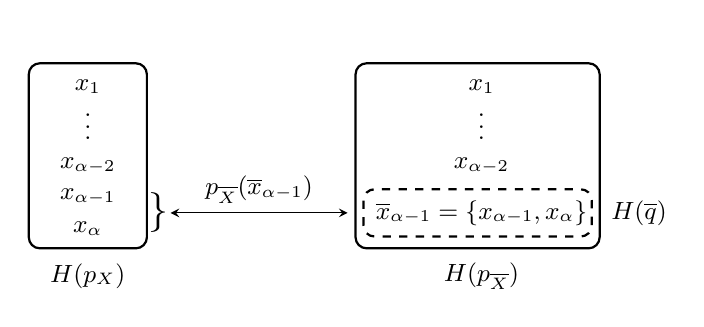
\begin{tikzpicture}
\shorthandoff{>}
%
% Ensemble \X
\draw(0,3) node{\small $\X$};
\draw(0,2.4) node{\small $x_1$};
\draw(0,2) node{\small $\vdots$};
\draw(0,1.4) node{\small $x_{\alpha-2}$};
\draw(0,1) node{\small $x_{\alpha-1}$};
\draw(0,.6) node{\small $x_{\alpha}$};
\draw(0,0) node{\small $H(p_X)$};
\draw[thick,rounded corners] (-.75,.35) rectangle (.75,2.7);
%
% Ensemble \overline{\X}
%
\draw(5,3) node{\small $\overline{\X}$};
\draw(5,2.4) node{\small $x_1$};
\draw(5,2) node{\small $\vdots$};
\draw(5,1.4) node{\small $x_{\alpha-2}$};
\draw(5,.8) node{\small $\overline{x}_{\alpha-1} = \{ x_{\alpha-1} , x_\alpha\}$};
\draw(5,0) node{\small $H(p_{\overline{X}})$};
\draw(7,.8) node{\small $H(\overline{q})$};
\draw[dashed,thick,rounded corners] (3.5,.5) rectangle (6.4,1.1);
\draw[thick,rounded corners] (3.4,.35) rectangle (6.5,2.7);
%
% juntando 2 estados VER PROBLEMA CON LA FLECHA
\draw(.9,.8) node{\Large $\}$};
\draw[>=stealth,<->] (1.05,.8)--(3.3,.8);
\draw (2.175,.8) node[above]{\small $p_{\overline{X}}(\overline{x}_{\alpha-1})$};
\end{tikzpicture} \end{center}
  %
  \leyenda{Ilustraci\'on de  la propiedad  de recursividad, que  cuantifica como
    decrece la entropia en un  conjunto cuando se juntan dos estados, vincluando
    la entropia  total, la  entropia despues del  la agrupaci\'on y  la entropia
    interna a los dos estados juntados.}
  %
  \label{fig:SZ:Recursividad}
  \end{figure}
%
\item\label{prop:SZ:concavidad} {\it Concavidad:} La  entropia es concava, en el
  sentido  de que  la entropia  de una  combinaci\'on convexa  de distribuciones
  (mezcla) de probabilidades es siempre major o igual a la combinaci\'on convexa
  de entropias:
  %
  \[
  \forall \: \{ \lambda_i \}_{i=1}^n, \quad  0 \le \lambda_i \le 1, \quad \sum_i
  \lambda_i = 1  \quad \mbox{and cualquier conjunto de  distribuciones} \quad \{
  p_i \}_{i=1}^n,
  \]
  %
  \[
  H\left(  \sum_i  \lambda_i p_i  \right)  \ge  \sum_i  \lambda_i H(p_i)
  \]
  %
  Esta desigualdad es conocida como  desigualdad de Jensen.  Es una consequencia
  directa de  la convexidad  de la funci\'on  $\phi: u  \mapsto u \log  u$, como
  ilustrado       en       la      figura~\ref{fig:SZ:Concavidad}-(a).        La
  figura~\ref{fig:SZ:Concavidad}-(b) ilustra como se puede obtener una mezcla de
  distribuciones  de  dos probabilidad  $p_1$  (dado  izquierda)  y $p_2$  (dado
  derecho)  haciendo una elecci\'on  aleatoria a  partir de  una moneda  en este
  ejemplo (probabilidad $\lambda$ de elegir el dado izquierda).\newline
  %
  \begin{figure}[h!]
  %
  \begin{center} \begin{tikzpicture}
\shorthandoff{>}
%
% Concavidad de - u log u
\begin{scope}[xscale=3,yscale=2.5]
\pgfmathsetmacro{\u}{.2};
\pgfmathsetmacro{\v}{1.25};
\pgfmathsetmacro{\l}{.7};
%
\draw[>=stealth,->] (-.5,0)--(1.6,0) node[right]{\small $u$};
\draw[>=stealth,->] (0,-.7)--(0,{1.5*log2(1.5)}) node[above]{\small $\phi(u) = u \log u$};
\draw[thick,domain=.005:1.5,samples=200] (0,0)-- plot (\x,{\x*log2(\x)});
\draw[dashed] (\u,{\u*log2(\u)})--(\v,{\v*log2(\v)});
\draw (\u,0)--(\u,-.05) node[below]{\small $u_1$};
\draw (\v,0)--(\v,-.05) node[below]{\small $u_2$};
%
\draw[dashed] ({\l*\u+(1-\l)*\v},.05) node[above]{\small $\lambda u_1 + (1-\lambda) u_2$}
--({\l*\u+(1-\l)*\v},{(\l*\u+(1-\l)*\v)*log2(\l*\u+(1-\l)*\v)});
%
% l phi(u) + (1-l) phi(v)
\draw[dotted]
({\l*\u+(1-\l)*\v},{\l*\u*log2(\u)+(1-\l)*\v*log2(\v)})--(-.05,{\l*\u*log2(\u)+(1-\l)*\v*log2(\v)})
node[left]{\small $\lambda \phi(u_1) + (1-\lambda) \phi(u_2)$};
%
% phi(l u + (1-l) v)
\draw[dotted]
({\l*\u+(1-\l)*\v},{(\l*\u+(1-\l)*\v)*log2(\l*\u+(1-\l)*\v)})--
(-.05,{(\l*\u+(1-\l)*\v)*log2(\l*\u+(1-\l)*\v)})
node[left]{\small $\phi(\lambda u_1 + (1-\lambda) u_2)$};
\end{scope}
%
%
% Concavidad / mezcla
\begin{scope}[xshift=8.5cm]
\draw(0,1.25) node{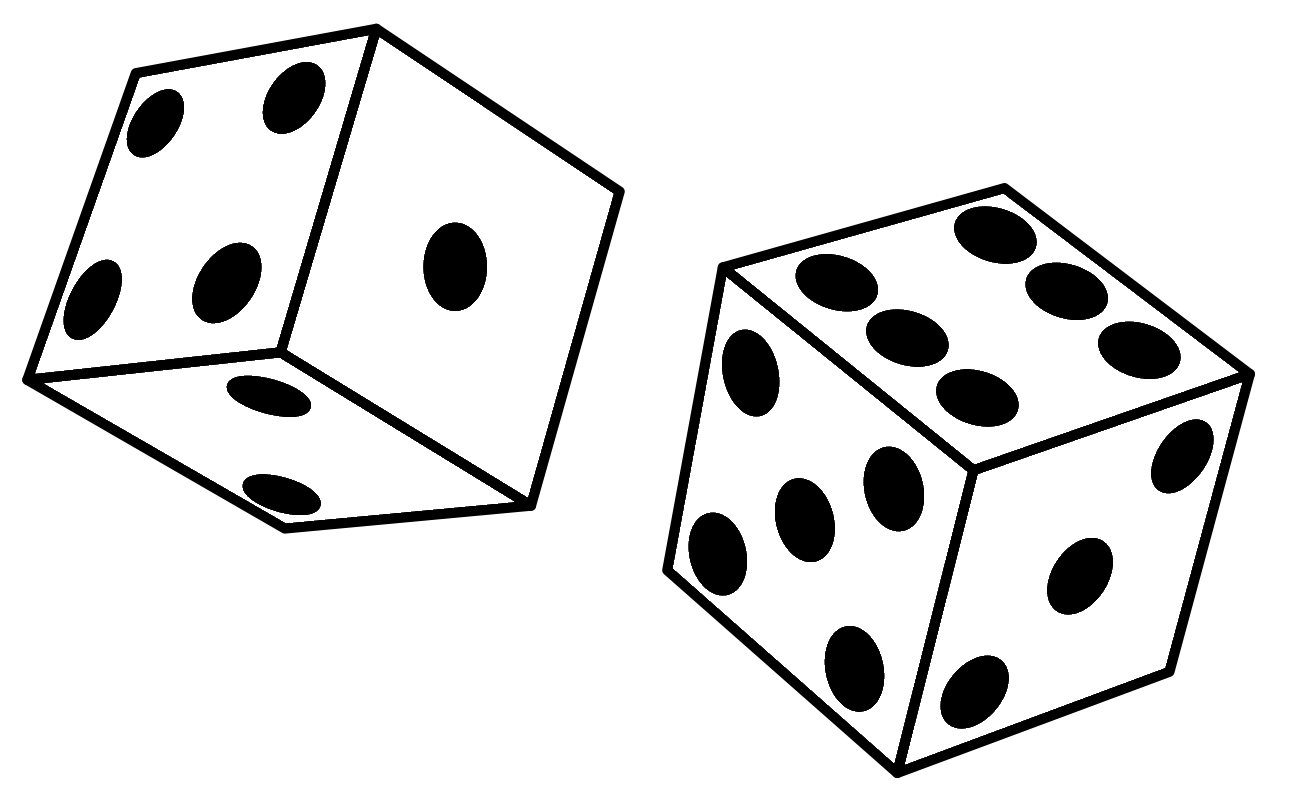
\includegraphics[width=3cm]{TIKZ_SZ/DosDados}};
\draw(-.5,2.5) node{\small $p_1$};
\draw(1,2) node{\small $p_2$};
\draw(2.7,1) node{\small $\lambda p_1 + (1-\lambda) p_2$};
\draw(-.25,-1) node{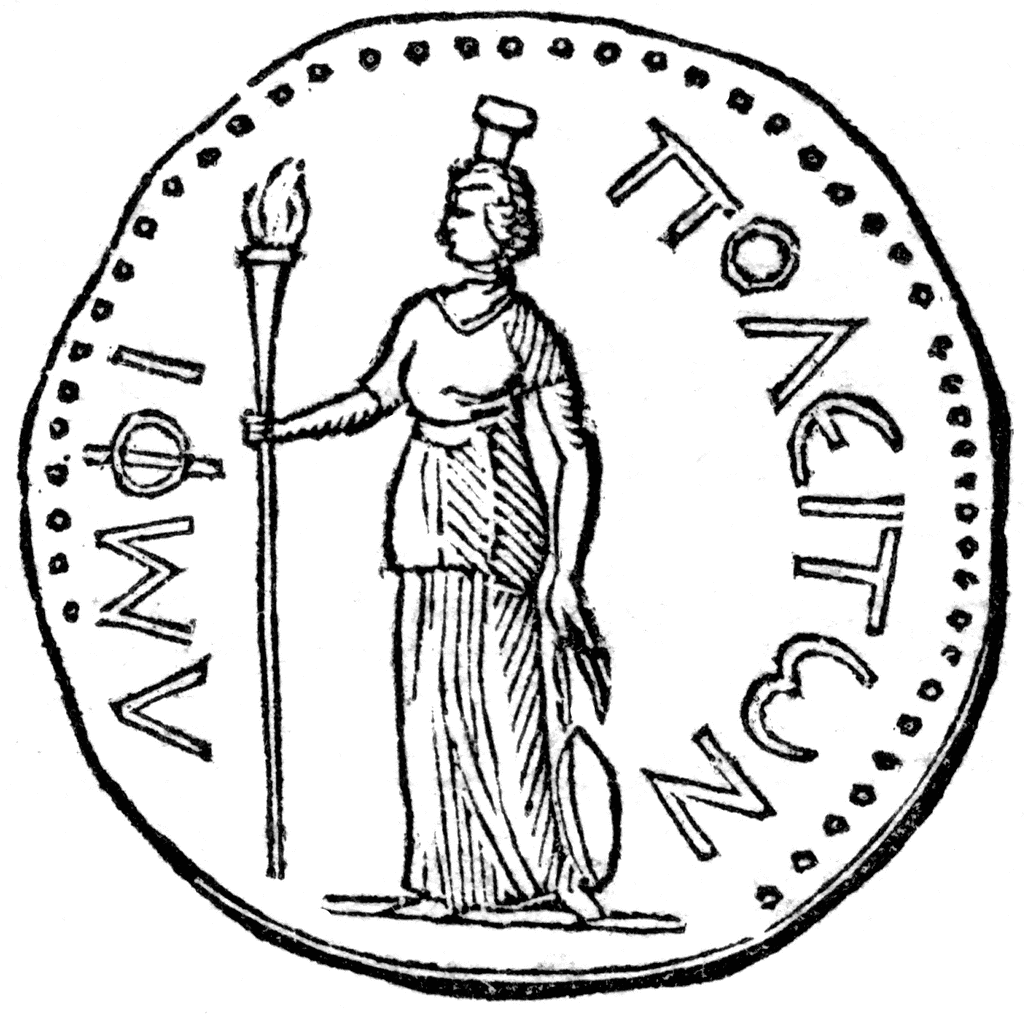
\includegraphics[width=1cm]{TIKZ_SZ/Moneda}};
\draw[>=stealth,->,thick] (-.3,-.35)--(-.75,.45);
\draw (-.525,0) node[left]{\small $\lambda$};
\draw[>=stealth,->,thick] (-.2,-.35)--(.3,.45);
\draw (.05,0) node[right]{\small $1-\lambda$};
\end{scope}
%
\draw (1.25,-2.25) node{(a)};
\draw (8.25,-2.25) node{(b)};
\end{tikzpicture} \end{center}
  %
  \leyenda{(a) $\phi(u)  = u \log u$ es  concava: la curva es  siempre debajo de
    sus cuerdas; entonces, cada promedio de $\phi(u_1)$ y $\phi(u_2)$ estando en
    la cuerda  juntando estos punto, queda  arriba de la funci\'on  tomada en el
    promedio de $u_1$  y $u_2$.  Escribiendo eso para (mas  de dos puntos) sobre
    los $\sum_i \lambda_i  p_i(x)$ y sumando sobre los $x$  da la desigualdad de
    Jensen.  (b) Ilustraci\'on de  una distribuci\'on de mezcla, ac\'a mezclando
    $p_1$  y  $p_2$  a  partir  de  una tercera  variable  aleatoria  (ac\'a  de
    Bernoulli).}
  %
  \label{fig:SZ:Concavidad}
  \end{figure}
%
\item\label{prop:SZ:Schurconcavidad}  {\it Schur-concavidad:}  Como se  lo puede
  querrer,  lo mas  ``concentrado'' es  una distribuci\'on  de  probabilidad, lo
  menos hay  incerteza, y entonces lo  mas peque\~no debe ser  la entropia. Esta
  propiedad intuitiva se resuma a partir de la noci\'on de mayorizaci\'on:
  %
  \begin{definicion}[Mayorizaci\'on]\label{def:SZ:Mayorizacion}
    Una distribuci\'on  discreta finita de probabilidad $p$  es dicha mayorizada
    por una distribuci\'on $q$,
    %
    \[
    p  \prec  q  \quad   \mbox{ssi}  \quad  \sum_{i=1}^k  p^\downarrow(x_i)  \le
    \sum_{i=1}^k q^\downarrow(x_i), \quad 1 \le  k < \alpha \quad \mbox{y} \quad
    \sum_{i=1}^\alpha p^\downarrow(x_i)  = \sum_{i=1}^\alpha q^\downarrow(x_i)
    \]
    %
    (las \'ultimas sumas siendo igual a 1).  Si los alfabetos de definici\'on de
    \ $p$ \ y  \ $q$ \ son de tama\~nos diferentes, \  $\alpha$ \ es el tama\~no
    lo  mas  grande y  la  distribuci\'on  sobre el  alfabeto  lo  mas corto  es
    completada por estados de probabilidad 0 (recuerdense de que no va a cambiar
    la entropia).
  \end{definicion}
  %
  La  Schur-concavidad  se  traduce  por  la  relaci\'on
  %
  \[
  p \prec  q \quad \Rightarrow  \quad H(p) \ge  H(q)
  \]
  %
  Fijense de que las cotas sobre $H$ pueden ser vistas como consecuencia de esta
  desiguldad:  la  distribuci\'on  cierta  mayoriza cualquier  distribuci\'on  y
  cualquier  distribuci\'on mayoriza  la distribuci\'on  uniforme.  \SZ{prueba a
    partir del teorema de Karamata?}
\end{propiedades}

En muchos  casos, uno tiene que  trabajar con varias  variables aleatorias. Para
simplificar les  notaciones, considera una par  de variables \  $X$ \ y \  $Y$ \
definidas respectivamente sobre los alfabetos \ $\X$  \ y \ $\Y$ \ de cardinal \
$\alpha = |\X|$ \ y \ $\beta =  |\Y|$.  Tal par de variable puede ser vista como
una  variable $(X,Y)$  definida sobre  el alfabeto  $\X \times  \Y$  de cardinal
$\alpha \beta$ tal  que se definie naturalmente la  entropia para esta variable;
tal entropia es llamada {\it entropia conjunta} de $X$ y $Y$:
%
%~\cite{Sha48, ShaWea64}
\begin{definicion}[Entropia conjunta]\label{def:SZ:EntropiaConjunta}
  Sean \ $X$ \ e \ $Y$  \ dos variable aleatorias definidas sobre los alpfabetos
  discretos \  $\X$ \ y \ $\Y$,  de cardinal \ $\alpha  = |\X| < +\infty$  \ y \
  $\beta  =   |\Y|  <  +\infty$  \   respectivamente.  Sea  \   $p_{X,Y}$  \  la
  distribuci\'on de probabilidad conjunta de \ $X$ \ e \ $Y$, \ \ie $ \forall \,
  (x,y) \in \X \times \Y, \quad p_{X,Y}(x,y) =  \Pr[X = x , Y = y]$. La entropia
  conjunta de Shannon de las variables \ $X$ \ e \ $Y$ \ es definida por
  %
  \[
  H(p_{X,Y}) =  H(X,Y) = -  \sum_{(x,y) \in \X  \times \Y} p_{X,Y}(x,y)  \, \log
  p_{X,Y}(x,y)
  \]
  %
  con la convenci\'on $0 \log 0 = 0$.
\end{definicion}

A partir de esta definici\'on,  aparecen otras propiedades importantes, sino que
fundamentales, de la entropia de Shannon.
%
\begin{propiedades}
\item\label{prop:SZ:aditividad}  {\it Aditividad:} La  entropia conjunta  de dos
  variables aleatorias  \ $X$  \ e \  $Y$ \underline{independientes} se  suma, y
  reciprocamente:
  %
  \[
  X \: \mbox{e} \: Y \: \mbox{independientes} \quad \Leftrightarrow \quad H(X,Y)
  =  H(X) +  H(Y)
  \]
  %
  Dicho de otra manera, para dos variables aleatorias, la incerteza global es la
  suma   de  las  incertezas   de  cada   variable  individual.    La  propiedad
  ``$\Rightarrow$'' es consecuencia directa de \ $p_{X,Y}(x,y) = p_X(x) p_Y(y)$.
  Se  va  a  probar  en  la  secci\'on siguiente  la  reciproca.  Se  generaliza
  sencillamente a un conjunto de variables aleatorias $\{ X_i \}$.
%
\item\label{prop:SZ:subaditividad} {\it Sub-aditividad:} La entropia conjunta de
  dos variables aleatorias  $\{ X_i \}_{i=1}^n$ es siempre menor  que la suma de
  cada entropia individual:
  %
  \[
  H(X_1,\ldots,X_n)  \,  \le \,  \sum_{i=1}^n  H(X_i)
  \]
  %
  Dicho de otra manera, variables  pueden compartir informaci\'on, de tal manera
  de que le entropia global sea menor que la suma.  De la propiedad anterior, se
  obtiene la igualdad ssi los $X_i$ son indepedientes.
%
\item\label{prop:SZ:superaditividad}   {\it   Super-aditividad:}   La   entropia
  conjunta de dos variables aleatorias  $\{ X_i \}_{i=1}^n$ es siempre major que
  cualquiera  de  las entropias  individuales
  %
  \[
  H(X_1,\ldots,X_n) \, \ge \, \max_{1 \le i \le n} H(X_i)
  \]
\end{propiedades}

Es importante notar  de que existen varios enfoques basados  sobre una series de
axiomas, dando lugar  a la definici\'on de la entropia  tal como definido. Estos
axiomas  son conocidos  como axiomas  de Shannon-Khinchin  y son  la continuidad
(propiedad~\ref{prop:SZ:continuidad}),               la              maximalidad
(propiedad~\ref{prop:SZ:cotamaxima}),              la             expansabilidad
(propiedad~\ref{prop:SZ:expansabilidad})         y         la         aditividad
(propiedad~\ref{prop:SZ:aditividad}).  Existen varios otros conjunto de axiomas,
conduciendo tambi\'en a la entropia de Shannon (ver Shannon~\cite[Sec.~6]{Sha48}
or    \cite{ShaWea64},    R\'enyi~\cite{Ren61},   Fadeev~\cite{Fad56,    Fad58},
Khintchin~\cite{Khi57} entre otros).

Para  una  serie de  variables  aleatorias,  $X_1,  X_2, \ldots$,  representando
simbolos, se puede  definir una entropia por simbolo  como una entropia conjunta
divido por numero de simbolos, $\frac{H(X_1,\ldots,x_n)}{n}$, as\'a que una taza
de entropia cuando $n$ va al inifinito.
%
\begin{definicion}[Taza de entropia]\label{def:SZ:TazaDeEntropia}
  Sea $\X = \{  X_i \}_{i \in \Nset^*}$ una  serie de variable aleatoria.  La taza de
  entropia de esta serie es definida por
  %
  \[
  \H(\X) = \lim_{n \to \infty} \frac{H(X_1,\ldots,X_n)}{n}
  \]
  %
\end{definicion}
%
\noindent Esta cantidad siempre existe, porque $H(X_1 , \ldots , X_n) \le \sum_i
H(X_i) \le \sum_i \log \alpha_i \le  n \max_i \alpha_i$ donde los $\alpha_i$ son
los cardinales de los alfabetos de definici\'on de los $X_i$.

\

Se termina esta sub-secci\'on con el caso de variables discretas definidas sobre
un  alfabeto $\X$ de  cardinal infinito  $|\X| =  + \infty$,  por ejemplo  $\X :
\Nset$.   Por  analogia,  se  puede  siempre  definir la  entropia  como  en  la
definici\'on Def.~\ref{def:SZ:Shannon}. Esta extensi\'on resuelta delicada dando
de que unas  propiedades se perdien.  Por ejemplo, la  entropia no queda acotada
por arriba  como se  lo puede  probar para la  distribuci\'on de  probabilidad \
$\displaystyle p(x)  \propto \frac{1}{(x+2) \left(  \log (x+2) \right)^2},  \: x
\in \Nset$, corectamente normalizada ($\propto$ significa ``proporcional a''): \
$\displaystyle \frac{\log \log(x+2)}{(x+2) \left( \log (x+2) \right)^2} \ge 0$ \
y  \  la  serie  \  $\displaystyle  \sum_x  \frac{1}{(x+2)  \log  (x+2)}$  \  es
divergente,  as\'i que  la serie  \ $\displaystyle  - \sum_x  p(x) \log  p(x)$ \
diverge.

% ================================= Axiomas

\subseccion{Entrop\'ia diferencial}
\label{sec:SZ:Diferencial}

Volviendo a la definici\'on Def.~\ref{def:SZ:Shannon} de la entropia de Shannon,
usando el operador $\Esp$ promedio  estadistica o esperanza matematica, se puede
rescribir la entropia de Shannon como $H(X) = \Esp\left[ - \log p_X(X) \right]$.
Con este punto  de vista, es facil extender la definici\'on  de la entropia para
variables aleatorias continuas admitiendo  una densidad de probabilidad.  Eso da
lugar a lo que es conocido como la {\it entropia diferencial}:

\begin{definicion}[Entropia diferencial]\label{def:SZ:EntropiaDiferencial}
  Sea $X$ una  variable aleatoria definida sobre un  espacio $d$-dimensional $\X
  \subseteq \Rset^d$ y sea $p_X(x)$ la densidad (distribuci\'on) de probabilidad
  de $X$, La entropia diferencial de la variable $X$ es definida por
  %
  \[
  H(p_X) = H(X) = - \int_\X p_X(x) \, \log p_X(x) \, dx
  \]
  %
  (con la  convenci\'on $0 \log  0 = 0$,  se puede escribir la  integraci\'on en
  $\Rset^d$).
\end{definicion}
%
Como en el  caso discreto, para $X = (X_1,\ldots,X_d)$, esta  entropia de $X$ es
dicha entropia conjunta de los componentes $X_i$.

Como se lo  va a ver, la entropia diferencial no  tiene la misma significaci\'on
de  incerteza,  siendo de  que  depende no  solamente  de  la distribuci\'on  de
probabilidad, sino que  de los estados tambi\'en.  Mas alla, no  se la puede ver
como l\'imite continua de un caso discreto:  a trav\'es de tal l\'imite, se va a
ver que se  llama diferencial, a causa del efecto de  la diferencial $dx$.  Para
ilustrar eso, considera una variable aleatoria  escalar \ $X$ \ viviendo sobre \
$\Rset$ \ y \  $p_X$ \ su densidad de probabilidad.  Sea \ $\delta  > 0$ \ y sea
el alfabeto $\X^\delta = \{ x_k \}_{k \in \Zset}$ \ donde los \ $x_k$ se definen
tal que  $\displaystyle p_X(x_k) \delta = \int_{k  \delta}^{(k+1) \delta} p_X(x)
\, dx$, como ilustrado  en la figure~\ref{fig:SZ:CuantificacionX}.  Se define la
variable  aleatoria discreta  \ $X^\delta$  \ sobre  \ $\X^\delta$  \ tal  que \
$\Pr[X^\delta =  x_k] = p_{X^\delta}(x_k) =  p_X(x_k) \delta$. \ Se  puede ver \
$X^\delta$ \ como la versi\'on cuantificada de \ $X$, \ con \ $X^\delta = x_k$ \
cuando  \ $X \in  [k \delta  , (k+1)  \delta )$.   \ Al  rev\'es, a\'un  que sea
delicado, se  puede interpretar \ $X$ \  como el ``l\'imite'' de  \ $X^\delta$ \
cuando \ $\delta$ \ tiende a 0. Ahora, es claro de que
%
\begin{eqnarray*}
H(X^\delta) & = & - \sum_k p_{X^\delta}(x_k) \log p_{X^\delta}(x_k)\\[2.5mm]
%
& = & - \log \delta - \sum_k \Big( p_X(x_k) \log p_X(x_k) \Big) \, \delta
\end{eqnarray*}
%
lo que se escribe tambien
%
\[
H(X^\delta)  + \log  \delta =  - \sum_k  \Big( p_X(x_k)  \log p_X(x_k)  \Big) \,
\delta
\]
%
Entonces, de la intergraci\'on de Rieman sale que
%
\[
\lim_{\delta \to 0} \left( H(X^\delta) + \log \delta \right) = H(X)
\]
%
Dicho de  otra manera,  la entropia  diferencial de $X$  no es  el limite  de la
entropia  de su  versi\'on  cuantificada:  aparece con  la  entropia el  termino
``diferencial'' $\log \delta$.
%
\begin{figure}[h!]
%
\begin{center} 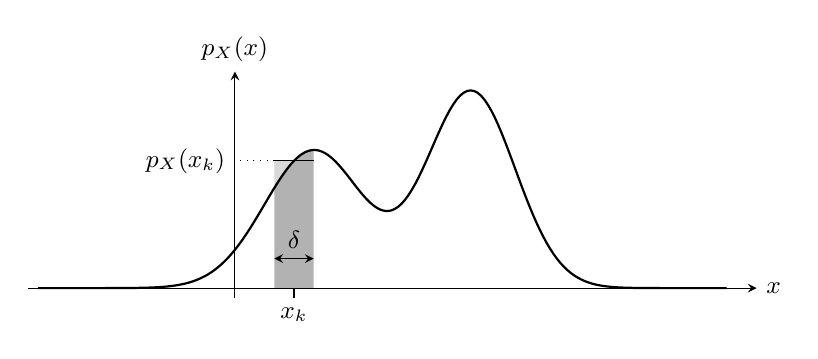
\begin{tikzpicture}
\shorthandoff{>}
%
% Cuantificacion de X
\begin{scope}[xscale=2.5,yscale=2.5]
%
\pgfmathsetmacro{\c}{.4};
\pgfmathsetmacro{\d}{1.2};
\pgfmathsetmacro{\s}{8};
\pgfmathsetmacro{\t}{10};
\pgfmathsetmacro{\a}{.7};
\pgfmathsetmacro{\b}{1};
%
\pgfmathsetmacro{\xk}{.3};
\pgfmathsetmacro{\dx}{.2};
%
\draw[>=stealth,->] (-1.05,0)--(2.65,0) node[right]{\small $x$};
\draw[>=stealth,->] (0,-.05)--(0,1.1) node[above]{\small $p_X(x)$};
%
% lei de proba
\draw[thick,domain=-1:2.5,samples=200] plot (\x,{(\a*exp(-\s*(\x-\c)^2)+\b*exp(-\t*(\x-\d)^2))});
%
% dominio alrededor de xk
\fill[domain=\xk-\dx/2:\xk+\dx/2,samples=20,opacity=.3]
({\xk-\dx/2},0)--
plot (\x,{(\a*exp(-\s*(\x-\c)^2)+\b*exp(-\t*(\x-\d)^2))})--
({\xk+\dx/2},0);
%
% xk y delta
\draw (\xk,0)--(\xk,-.05) node[below]{\small $x_k$};
\draw[>=stealth,<->] ({\xk-\dx/2},.15)--({\xk+\dx/2},.15);
\draw (\xk,.15) node[above]{\small $\delta$};
%
% recta sobre delta a altura de p(xk)
\draw ({\xk+\dx/2},{(\a*exp(-\s*(\xk-\c)^2)+\b*exp(-\t*(\xk-\d)^2))})--
({\xk-\dx/2},{(\a*exp(-\s*(\xk-\c)^2)+\b*exp(-\t*(\xk-\d)^2))});
\draw[dotted] ({\xk-\dx/2},{(\a*exp(-\s*(\xk-\c)^2)+\b*exp(-\t*(\xk-\d)^2))})--
(0,{(\a*exp(-\s*(\xk-\c)^2)+\b*exp(-\t*(\xk-\d)^2))}) node[left]{\small $p_X(x_k)$};
%
% dominio equivalente alrededo de xk
\fill[domain=\xk-\dx/2:\xk,samples=20,opacity=.15]
plot (\x,{(\a*exp(-\s*(\x-\c)^2)+\b*exp(-\t*(\x-\d)^2))})--
({\xk-\dx/2},{(\a*exp(-\s*(\xk-\c)^2)+\b*exp(-\t*(\xk-\d)^2))});
\end{scope}
\end{tikzpicture} \end{center}
%
\leyenda{Densidad de probabilidad $p_X$ de $X$, construcci\'on del alfabeto $\X$
  donde  se  define   la  versi\'on  cuantificada  $X^\delta$  de   $X$  con  su
  distribuci\'on discreta de probabilidad $p_{X^\delta}$. La superficia en grise
  oscuro es igual a la superficia definida por el rectangulo en grise claro.}
%
\label{fig:SZ:CuantificacionX}
\end{figure}
%

Mas  all\'a  de  esta  notable  diferencia  entre  la  entropia  y  la  entropia
diferencial, la \'ultima depende de los estados,  es decir que si $Y = g(X)$ con
$g$  biyectiva,  no  se  conserva  la  entropia,  \ie  \underline{se  pierde  la
  propiedad~\ref{prop:SZ:biyeccion}}  del  caso discreto:
%
\begin{eqnarray*}
H(Y) & = & - \int_{\Rset^d} p_Y(y) \log p_Y(y) \, dy\\[2.5mm]
%
& = &  - \int_{\Rset^d} p_Y(g(x)) \log p_Y(g(x)) \, |\Jac_g(x)| \, dx\\[2.5mm]
%
& = & - \int_{\Rset^d} p_Y(g(x)) \Big( \log \big( p_Y(g(x)) \, |\Jac_g(x)| \big) -
\log |\nabla^t g(x)| \Big) \, |\Jac_g(x)| \, dx
\end{eqnarray*}
%
donde $\Jac_g$ es la  matriz de componentes $\frac{\partial g_i}{\partial x_j}$,
Jacobiano  de  la  transformaci\'on  \   $g:  \Rset^d  \mapsto  \Rset^d$  \  ($g
\equiv  \begin{bmatrix} g_1(x_1  ,  \ldots  , x_d)  &  \cdots &  g_d(x_1  , \ldots  ,
  x_d)  \end{bmatrix}^t$) \  y  \  $|\cdot|$ representa  el  valor absoluto  del
determinente   de  la  matriz.    Recordandose  de   que  $p_X(x)   =  p_Y(g(x))
|\Jac_g(x)|$, se obtiene
%
\begin{propiedadesC}\setcounter{enumi}{\value{PropBiyeccion}}
%
\item\label{prop:SZ:biyeccionC}
Para  cualquier biyecci\'on $g:  \Rset^d \mapsto  \Rset^d$
  %
  \[
  H(g(X)) = H(X) + \int_{\Rset^d} p_X(x) \log |\Jac_g(x)| \, dx
  \]
  %
  donde el \'ultimo termino, $\Esp\left[  \log |\Jac_g(X)| \right]$ no vale cero
  en    general.   En    particular,   si    $H$   es    invariante    bajo   un
  deplazamiento,
  %
  \[
  H(X+\mu) = H(X) \quad \forall \: \mu \in \Rset^d
  \]
  %
  no  es invariante  por cambio  de escala,
  %
  \[
  H(a X) = H(X) + \log |a| \quad \forall \: a \in \Rset^*
  \]
\end{propiedadesC}
%
Esta  \'ultima relaci\'on  queda valid  para  $a$ matriz  invertible.  Por  esta
\'ultima  relaci\'on, se puede  ver que,  dado $X$,  cuando $a$  tiende a  0, la
entropia de  $a X$ tiende a  $-\infty$.  Es decir que,  para $a$ suficientemente
peque\~no,  se  puede  tener $H(a  X)  <  0$,  as\'i que  \underline{se  pierde}
tambi\'en \underline{la positividad, propiedad~\ref{prop:SZ:positividad}}.  Esta
perdida definitivamente quita la interpretaci\'on de incerteza/informaci\'on que
hubiera podido tener la entropia diferencial.  A veces, se usa lo que es llamado
potencia entropica:
%
\begin{definicion}[Potencia entropica]
  Sea $X$ una  variable aleatoria $d$-dimensional. La potencia  entropica de $X$
  es definida por
  %
  \[
  N(X) = \frac{1}{2 \pi \e} \exp\left( \frac2d H(X) \right)
  \]
\end{definicion}
%
\noindent Por construcci\'on,  $N(X) \ge 0$.  Ademas, en  el caso continuo, $N(a
X+b) = |a|^2 N(X)$ (queda valida para una matriz $a$ invertible): esta propiedad
puede justificar la idea de  ``potencia''; ademas $N(a X+b)$ tiende naturalmente
a cero cuando $a$ tiende a  cero.  Se recupera as\'i la noci\'on informacional a
trav\'es  de  $N$ en  este  contexto  ($a X  +  b$  ``tiende''  a $b$,  variable
deterministica).

Si se pierde  la propiedad de invarianza bajo  una biyecci\'on, sopredentemente,
se conserva la entropia bajo el equivalente continuo del rearreglo.
%
\begin{definicion}[Rearreglo simetrico]
  Sea $\P \subset \Rset^d$ abierto de  volumen finito $|\P| < +\infty$.  El {\it
    rearreglo simetrico}  $\P^\downarrow$ de  $\P$ es la  bola centrada en  0 de
  mismo volumen  que $\P$, \ie
  %
  \[
  \P^\downarrow  = \left\{  x  \in  \Rset^d \,  :  \: \frac{2  \pi^{\frac{d}{2}}
      |x|^d}{\Gamma\left(\frac{d}{2}\right)} \le |\P| \right\}
  \]
  %
  donde   $|\cdot|$   denota   la    norma   euclideana.    Eso   es   ilustrado
  figure~\ref{fig:SZ:ensemblerearreglado}-a.\newline  Sea $p_X$ una  densidad de
  probabilidad y sea $\P_t = \{ y \, : \: p_X(y) > t \}$ para cualquier $t > 0$,
  sus conjuntos  de niveles.  La densidad de  probabilidad~\footnote{Se proba de
    que  esta funci\'on,  positiva  por  definici\'on, suma  a  1.  Ademas,  por
    construcci\'on,  depende   unicamente  de   $|x|$  y  decrece   con  $|x|$.}
  rearreglada simetrica $p^\downarrow_X$ de $p_X$ es definida por
  %
  \[
  p^\downarrow_X(x)  =  \int_0^{+\infty}  \un_{\P_u^\downarrow}(x) \,  du
  \]
  %
  con $\un_A$ el indicator  del conjunto $A$, \ie $\un_A(x) = 1$  si $x \in A$ y
  cero sino.
\end{definicion}
%
Del hecho  de que $\forall \, t  < \tau \: \Leftrightarrow  \: \P_\tau \subseteq
\P_t  \:  \Leftrightarrow \:  \P_\tau^\downarrow  \subseteq \P_t^\downarrow$  es
sencillo   ver   que   si   $x   \in  \P_\tau^\downarrow$,   entonces   $x   \in
\P_t^\downarrow$, lo que conduce a  $p_X^\downarrow(x) > \tau$ y vice-versa. Mas
alla,  sobre $\P_{\tau+d\tau}  \backslash \P_\tau$  la funci\'on  $p_X$ ``vale''
$\tau$ \ y \ sobre $\P_{\tau+d\tau}^\downarrow \backslash \P_\tau^\downarrow$ la
funci\'on $p_X^\downarrow$  ``vale'' tambien $\tau$, lo que  da \ $\displaystyle
\int_{\P_\tau^\downarrow} p_X^\downarrow(x) \, dx = \int_{\P_\tau} p_X(x) \, dx$
(ver~\cite{LieLos01, WanMad04} para une prueba mas rigorosa).  La representaci\'on de la
definici\'on es conocida como representaci\'on en capas de pastel (layer cake en
ingles). Eso es ilustrado en la figura~\ref{fig:SZ:ensemblerearreglado}-b
  %
  \begin{figure}[h!]
  %
  \begin{center} 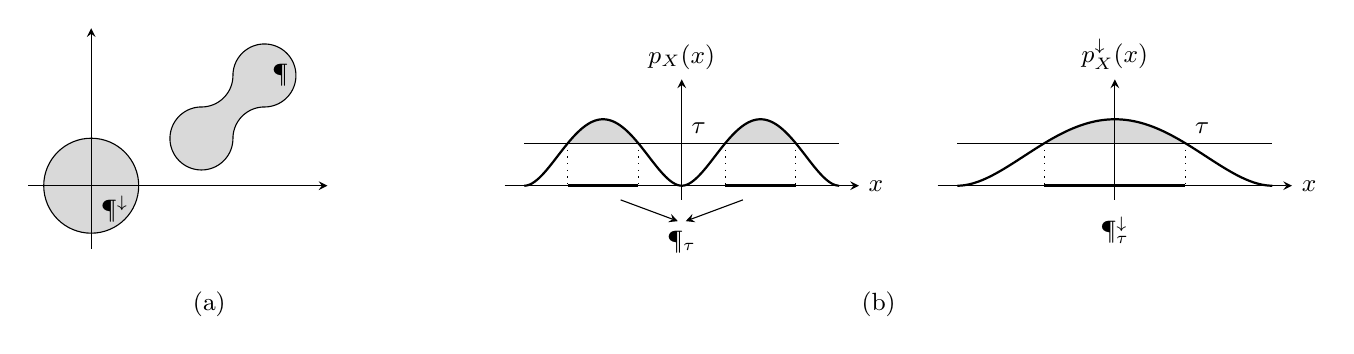
\begin{tikzpicture}
\shorthandoff{>}
%
\begin{scope}[scale=.4]
% Superficia 2*3 pi/4  + 2*2 - 2*pi/4 = 4+pi
\filldraw[draw=black,fill=gray!30]
   plot [domain=0:-270,samples=200] ({cos(\x)+3.5},{sin(\x)+1.5})
-- plot [domain=-90:0,samples=200] ({cos(\x)+3.5},{sin(\x)+3.5})
-- plot [domain=180:-90,samples=200] ({cos(\x)+5.5},{sin(\x)+3.5})
-- plot [domain=90:180,samples=200] ({cos(\x)+5.5},{sin(\x)+1.5})
-- cycle;
\draw (6,3.5) node {\small $\P$};
%
% superficia rearreglada
\filldraw[draw=black,fill=gray!30] (0,0) circle ({sqrt(1+4/pi)});
\draw (.75,-.75) node {\small $\P^\downarrow$};
%
% ejes
\draw[>=stealth,->] (-2,0)--(7.5,0);
\draw[>=stealth,->] (0,-2)--(0,5);
%
\end{scope}
%
%
%----------------------------------------
%
% p_X(x), P_tau...
\begin{scope}[xshift=7.5cm,yscale=1.8]
\pgfmathsetmacro{\t}{.3};
\pgfmathsetmacro{\xt}{sqrt(1-sqrt(32*\t/15))};
\pgfmathsetmacro{\dx}{5.5};% shift para p*(x)
%
% mezcla de Student-r 15/16 * (1-x^2)^2 (nu = 5) centrados en -1 y 1
% 15/32 (1-(x-a)^2)^2 > t iif (x-a)^2 < 1-sqrt(32*t/15)
% i.e. a-sqrt(1-sqrt(32*t/15)) < x < a+sqrt(1-sqrt(32*t/15))
\fill[domain=-1-\xt:-1+\xt,fill=gray!30] plot(\x,{(15/32)*(1-(\x+1)^2)^2}); % p(x) > tau, x < 0 
\fill[domain=1-\xt:1+\xt,fill=gray!30] plot(\x,{(15/32)*(1-(\x-1)^2)^2}); % p(x) > tau, x > 0
\draw[thick,domain=-2:0,samples=100] plot(\x,{(15/32)*(1-(\x+1)^2)^2}); % p(x), x < 0
\draw[thick,domain=0:2,samples=100] plot(\x,{(15/32)*(1-(\x-1)^2)^2}); % p(x), x > 0
\draw (-2,\t)--(2,\t); \draw (0,\t) node[above right]{\small $\tau$}; % y = tau
%
% dominio P_tau
\draw[dotted] ({-1-\xt},{(15/32)*(1-\xt^2)^2})--({-1-\xt},0);
\draw[dotted] ({-1+\xt},{(15/32)*(1-\xt^2)^2})--({-1+\xt},0);
\draw[very thick] ({-1-\xt},0)--({-1+\xt},0);
\draw[>=stealth,->] ({-1+\xt/2},-.1)--(-.05,-.25);
%
\draw[dotted] ({1-\xt},{(15/32)*(1-\xt^2)^2})--({1-\xt},0);
\draw[dotted] ({1+\xt},{(15/32)*(1-\xt^2)^2})--({1+\xt},0);
\draw[very thick] ({1-\xt},0)--({1+\xt},0);
\draw[>=stealth,->] ({1-\xt/2},-.1)--(.05,-.25);
%
\draw (0,-.25) node[below]{\small $\P_\tau$};
%
% ejes
\draw[>=stealth,->] (-2.25,0)--(2.25,0) node[right]{\small $x$};
\draw[>=stealth,->] (0,-.1)--(0,.75) node[above]{\small $p_X(x)$};
%
%---------------------------
%
% 15/32 (1-(x-a)^2)^2 > t iif (x-a)^2 < 1-sqrt(32*t/15)
% i.e. a-sqrt(1-sqrt(32*t/15)) < x < a+sqrt(1-sqrt(32*t/15))
% Volumen 2*sqrt(1-sqrt(32*t/15))
% Por simetria, P_t* = [-2*sqrt(1-sqrt(32*t/15)) , 2*sqrt(1-sqrt(32*t/15))]
% da f*(x) = 15/32 (1-x^2/4)^2
\fill[domain=-2*\xt:2*\xt,fill=gray!30] plot({\x+\dx},{(15/32)*(1-.25*abs(\x)^2)^2}); % p*(x) > tau
\draw[thick,domain=-2:2,samples=200] plot({\x+\dx},{(15/32)*(1-.25*abs(\x)^2)^2});
\draw ({-2+\dx},\t)--({2+\dx},\t); \draw ({2*\xt+\dx},\t) node[above right]{\small $\tau$}; % y = tau
%
% dominio P_tau*
\draw[dotted] ({-2*\xt+\dx},{(15/32)*(1-\xt^2)^2})--({-2*\xt+\dx},0);
\draw[dotted] ({2*\xt+\dx},{(15/32)*(1-\xt^2)^2})--({2*\xt+\dx},0);
\draw[very thick] ({-2*\xt+\dx},0)--({2*\xt+\dx},0);
%
\draw (\dx,-.15) node[below]{\small $\P_\tau^\downarrow$};
%
% ejes
\draw[>=stealth,->] ({-2.25+\dx},0)--({2.25+\dx},0) node[right]{\small $x$};
\draw[>=stealth,->] (\dx,-.1)--(\dx,.75) node[above]{\small $p_X^\downarrow(x)$};
\end{scope}
%
\draw (1.5,-1.5) node{\small (a)};
\draw (10,-1.5) node{\small (b)};
\end{tikzpicture} \end{center}
  %
  \leyenda{(a):  Ilustraci\'on  del rearreglo  simetrico  $\P^\downarrow$ de  un
    conjunto  $\P$,  siendo  la  bola  centrada  en 0  de  mismo  volumen.   (b)
    Construcci\'on  del rearreglo  $p_X^\downarrow$:  dado un  $\tau$, se  busca
    $\P_\tau$ y  se deduce $P_\tau^\downarrow$; dado  un $x$, se  busca el mayor
    $t$  tal  que  $x  \in  P_t^\downarrow$, este  $t$  maximo  siendo  entonces
    $p_X^\downarrow(x)$;  ademas, por construcci\'on,  las superficias  en grise
    son iguales.}
  %
  \label{fig:SZ:ensemblerearreglado}
  \end{figure}
% =  \B  \left( 0  , r_\P  \right)$ con  $\frac{2
%    \pi^{d/2} r_\P^d}{\Gamma(d/2)} = |\P|$.

\begin{propiedadesC}\setcounter{enumi}{\value{PropPermutacion}}
\item\label{prop:SZ:permutacionC} {\it invarianza  bajo un rearreglo:} Sea $p_X$
  densidad   de  probabilidad   sobre   un  abierto   de  $\Rset^d$,
  %
  \[
  H\left( p_X^\downarrow \right) = H(p_X)
  \]
\end{propiedadesC}
%
\noindent Esta propiedad es probada por ejemplo en~\cite{LieLos01, WanMad04}.

\SZ{A ver que pasa en termino de mayorizacion~\ref{prop:SZ:mayorizacion}?}

Como  se lo  ha visto,  la  entropia diferencial  no es  siempre positiva,  como
consecuencia  de~\ref{prop:SZ:biyeccionC}.   Tambi\'en,  la  propiedad  de  cota
superior,  \underline{propiedad~\ref{prop:SZ:cotamaxima} se pierde}  en general,
\underline{salvo si se pone vinculos}:
%
\begin{propiedadesC}\setcounter{enumi}{\value{PropCotamaxima}}
\item
  \begin{enumerate}
  \item\label{prop:SZ:cotamaximauniforme} Si $\X$ es de volumen finito $|\X| < +
    \infty$, la entropia es acotada por arriba,
    %
    \[
    H(X) \le \log |\X|
    \]
    %
    con igualdad ssi $X$ es \underline{uniforme}.
    %
  \item\label{prop:SZ:cotamaximagaussiana}  Si  $\X =\Rset^d$  y  $X$ tiene  una
    matriz  de covarianza  dada  $\Sigma_X  = \Esp\left[  X  X^t \right]$  donde
    $\cdot^t$  denota  la transpuesta,  la  entropia  es  tambi\'en acotada  por
    arriba,
    %
    \[
    H(X) \le \frac{d}{2} \log(2 \pi \e) + \frac12 \log |\Sigma_X|
    \]
    %
    con igualdad  ssi $X$ es \underline{gaussiana}.  En  particular, la potencia
    entropica de  la gaussiana vale $N(X) =  \left| \Sigma_X \right|^{\frac1d}$,
    dando de nuevo un  ``sabor'' de potencia a $N$.  Como se o  va a ver en este
    cap\'itulo,  la  gaussiana  juega  un   rol  central  en  la  teoria  de  la
    informaci\'on.
  \end{enumerate}
  En  ambos casos,  estas  desigualdades con  la  distribuci\'on maximizante  se
  obtienen resolviendo  el problema de  maximizaci\'on de la entropia  subjeto a
  vinculos.      Se     trata    del     caso     m\'as     general    en     la
  secci\'on~\ref{sec:SZ:MaxEnt}.
\end{propiedadesC}

Al      final,     \underline{se      conservan      las     propiedades      de
  concavidad~\ref{prop:SZ:concavidad},  de aditividad~\ref{prop:SZ:aditividad} y
  de sub-aditividad~\ref{prop:SZ:subaditividad}}.   Es interesante de  notar que
de  la desigualdad~\ref{prop:SZ:subaditividad},  puramente  entropica, se  puede
deducir la  desigualdad de Hadamard,  desigualdad puramente matricial:  $|R| \le
\prod_i  R_{i,i}$  para  cualquier  matriz simetrica  definida  positiva  (viene
de~\ref{prop:SZ:subaditividad} escrita  para una  gaussiana de covarianza  $R$ y
tomando una exponencial de la desigualdad).